% !TEX root = ../IS.tex
\chapter{Introduction}
As the computing power of personal computers has increased, the depth and variety of interactive computer games has similarly increased. The earliest video games - \textit{Spacewar!} (1962) and \textit{Pong} (1972), for example - required two human players, and did not have any digital opponents. By the late 70's, games like \textit{Pursuit} (1975), \textit{Space Invaders} (1978), and \textit{Asteroids} (1979) introduced computer-controlled opponents which moved in set patterns.\\

\begin{figure}[H]
  \centering
  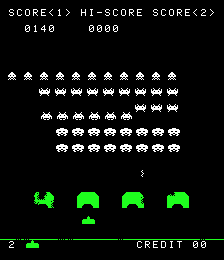
\includegraphics[width=9cm]{figures/space-invaders.png}
  \caption{A screenshot from the game \textit{Space Invaders}. The top line of enemy ships has reached the left side of the screen, so all enemy ships are in the midst of advancing forward \cite{spaceinvaders78}.}
  \label{fig:SpaceInvaders}
\end{figure}

In Space Invaders, enemies move in horizontal lines and occasionally shoot at the player, as shown in Figure \ref{fig:SpaceInvaders}. The player can move horizontally, to dodge projectiles and hide behind shields, and shoot back at the enemy. When a line of enemies hits a wall, the ships advance toward the player. As more enemy ships are destroyed, the lines become faster and faster, making them harder to hit. If a ship advances all the way to the player, the game ends and the player loses. Although the game becomes more difficult as the game progresses - ships become faster and shields become damaged - this difficulty has little to do with decisions made by the enemy ships; they just continue moving across the screen and shooting wildly.\\

\begin{figure}[H]
  \centering
  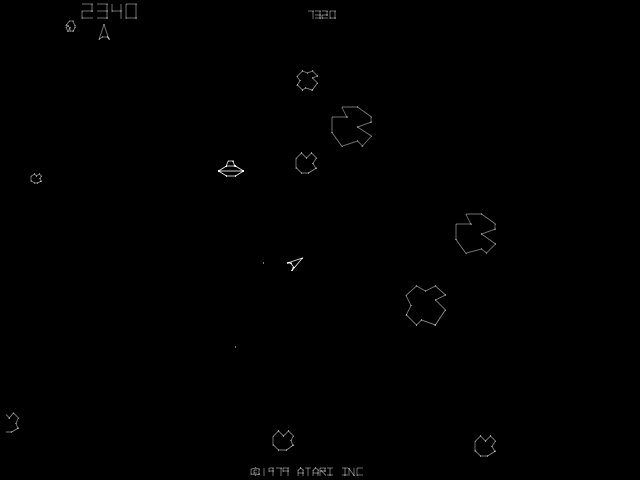
\includegraphics[width=9cm]{figures/Asteroids.png}
  \caption{A screenshot from the game \textit{Asteroids}. The player controls the triangular ship, and the flying saucer shoots in random directions. Another type of saucer exists in the game which fires directly at the player \cite{asteroids79}.}
  \label{fig:Asteroids}
\end{figure}

In Asteroids, the player's ship is freely movable in space. The ship must avoid or destroy asteroids and two different types of flying saucers. One saucer, the larger of the two, fires shots randomly. The other, smaller saucer targets the player directly and fires at them. In addition, the asteroids break into smaller asteroids as the player shoots them. Again, the difficulty of the game increases as asteroids break into smaller, faster pieces, but this does not reflect any choices made by the asteroids. The asteroids themselves simply move as the law of inertia dictates. Only the second saucer, which directly targets the player, has a semblance of intelligence. We infer from the nature of the gameplay that the saucer wants to destroy the player. By shooting right at the player, this enemy takes steps to achieve this goal. In contrast, the saucer which shoots randomly will sometimes try to achieve their goal (when the randomly-fired projectile moves in the general direction of the player) and sometimes will not (when the projectile moves in the complete opposite direction).\\

As time progressed, the intelligence of these enemies was improved with more intricate patterns (as in the space shooter Galaga (1981)) or in more heavily-scripted responses to inputs (as in the first-person shooter Half-Life (1998)) \cite{schw04}.
\begin{figure}[H]
  \centering
  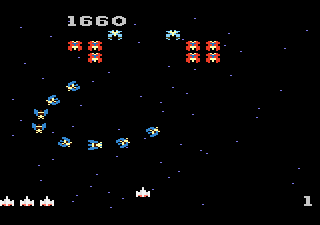
\includegraphics[width=8cm]{figures/ExampleGalaga.png}
  \caption{Four screenshots from the game \textit{Galaga}, showcasing (from 1 to 4) the movement of enemy ships \cite{galaga81}.}
  \label{fig:Galaga}
\end{figure}
Galaga, for example, uses curves and loops in the flight paths of enemy spaceships, as can be seen in Figure \ref{fig:Galaga}. Compared to the straight lines of \textit{Space Invaders}, the spaceships became more challenging to hit. Furthermore, the spaceships were programmed to fire when the player was directly below them, while \textit {Space Invaders} had enemies shooting seemingly at random \cite{schw04}.\\

In more recent titles, AI systems begin to show more intelligence. Some of this comes from more complex routines, as seen in the final boss of the game \textit{Final Fantasy IX}.

\lstset{caption={Section of AI script for Necron, an enemy in the game \textit{Final Fantasy IX} \protect\cite{ff9necron}.}, language=ff9code, label={lst:ff9Necron}}
\begin{lstlisting}
  set selectedattack = RandomAttack( attacklist )
  if ( selectedattack == Flare )
  set SV_Target = RandomInTeam( NotMatching(SV_PlayerTeam[STATUS_CURRENT], PETRIFY | DEATH | ZOMBIE | REFLECT) & NotMatching(SV_PlayerTeam[STATUS_AUTO], REFLECT) )
  elseif ( selectedattack == Holy )
  set SV_Target = RandomInTeam( NotMatching(SV_PlayerTeam[STATUS_CURRENT], PETRIFY | DEATH | ZOMBIE | REFLECT) & NotMatching(SV_PlayerTeam[STATUS_AUTO], REFLECT) )
  elseif ( selectedattack == Meteor )
  set SV_Target = SV_PlayerTeam
\end{lstlisting}

The boss, named Necron, has a variety of possible actions, three of which are shown in Listing \ref{lst:ff9Necron}. A random attack is selected from the list in line 1. For two of these attacks, a random character in the player's team is selected, provided that they do not have one of the listed special statuses, in lines 3 and 5. Two of these statuses (PETRIFY and DEATH) refer to when a character controlled by the player can no longer perform actions of their own \cite{ffIX00}. In this case, Necron targets a random character in the player's party who is not petrified or dead. The REFLECT status, on the other hand, prevents a player character from being affected by magic spells; the spells are reflected back at the opponent instead \cite{ffIX00}. For instance, if Necron did not exclude characters with the REFLECT status and tried to cast its Holy or Flare spell on a character with REFLECT, the spell would not damage said character. Instead, Holy or Flare would be reflected and deal damage to Necron, effectively causing the boss to damage itself. Thus, by excluding characters with REFLECT from the list of possible targets, Necron avoids making costly mistakes in battle. These checks improve the perceived ``intelligence'' of the boss; the AI does not waste actions attacking incapacitated players or causing itself harm from reflected magic.\\

While the \textit{Final Fantasy IX} example employs predetermined choices (apart from some random selection), other forms of intelligence come from more open-ended coding. For example, stealth games feature guards who must react to a variety of situations. One technique for such AI is to use fuzzy logic \cite{schw04}. Fuzzy logic deals with sets where membership is on a continuum \cite{zade65}. In this case, a guard in a stealth game would use this type of logic to transition from a calm state to a suspicious state to an alerted state as the player's presence is detected \cite{schw04}. Fuzzy logic is essential in this case to account for distance; if a player makes noise two rooms away, the guard shouldn't have as strong a reaction as when a player makes noise directly behind a guard. But, since a player may intentionally create distractions to exploit this suspicion, the AI for that guard cannot be too strongly scripted; what one player may do as a distraction another player may do accidentally, and the AI must account for these differences in play.\\

In many role-playing games (RPGs) like \textit{Final Fantasy IX}, the heroes live in fantastical worlds and often have the ability to heal themselves of their wounds with a quick potion or magic spell. While the player-controlled characters have these abilities, their AI-controlled opponents frequently do not. In rare cases where these enemies can heal themselves, this ability is often relegated to one-time uses determined by the game designers. For instance, an enemy may heal itself when it is close to death, but only the first time. When said enemy is once again close to death, they will not attempt to heal again. The goal of an opponent in a role-playing game should be survival, yet their choice to only heal once does not support that goal.\\

In order to make an AI opponent in a role-playing game which displays intelligence, the opponent should not be unduly limited in its ability to heal. This thesis concerns itself with designing an AI that can decide when to use a healing ability, and using game theory to analyze the effectiveness of an AI's strategy.